\newgeometry{left=1in, right=1in, top=1in, bottom=1.2in}

\chapter{Introduction}
\section{Project Overview}
Medical insurance cost prediction is a practical supervised learning problem that combines demographic, behavioral, and health-related information to estimate the amount an individual may be charged by an insurer. In this project, a regression-based workflow was developed and evaluated on the medical insurance dataset to predict insurance charges accurately while also identifying the most influential factors behind cost variation.

The dataset contains 1,338 records and seven variables, including both numerical and categorical attributes. The target variable, \textit{charges}, is continuous and strongly skewed, which makes regression modelling particularly relevant. The objective of this study is not only to produce accurate predictions but also to understand which factors drive insurance premiums and how different regression algorithms perform under the same data conditions.

\section{Objectives}
The main objectives of this study were to:
\begin{itemize}
  \item build a reliable predictive model for insurance cost estimation;
  \item compare multiple regression approaches under a consistent evaluation framework;
  \item identify the key variables that influence insurance charges; and
  \item present the workflow and outcomes in a structured and professional report.
\end{itemize}

\chapter{Dataset and Methodology}
\section{Dataset Description}
The dataset used in this study contains information about individuals including age, sex, body mass index (BMI), number of children, smoking status, residential region, and the corresponding insurance charges. These variables are suitable for supervised regression because they provide a mix of continuous and categorical predictors that can influence the insurance premium.

The dataset was reviewed for completeness and consistency before modelling. No missing values were detected, which simplified the preprocessing stage. Since several features were categorical, encoding was required before training the models that rely on numerical input matrices.

\section{Preprocessing and Experimental Setup}
The experimental workflow included the following steps:
\begin{enumerate}
  \item loading the dataset and examining its structure;
  \item transforming categorical variables into numerical representations;
  \item splitting the data into training and test sets using an 80/20 ratio;
  \item training several regression models on the training subset; and
  \item evaluating each model on the held-out test set using regression metrics such as MAE, RMSE, and $R^2$.
\end{enumerate}

The modelling strategy was designed to compare both tree-based methods and linear regularised approaches. This allowed the study to assess whether the relationship between predictors and charges is best captured by non-linear interactions or by a simpler linear structure.

\chapter{Exploratory Data Analysis}
\section{Distribution of Variables}
A preliminary exploratory analysis revealed that the target variable, insurance charges, is highly right-skewed. This suggests that a small number of observations have substantially higher costs than the majority of the sample. Such skewness is common in insurance data and can affect the behaviour of optimisation-based models if not handled carefully.

The distributions of age, BMI, and the number of children were also examined to understand whether they showed meaningful patterns relative to the target variable. The visual inspection indicated that smoking status is strongly associated with higher insurance charges, while other attributes appear to have weaker or more indirect relationships.

\begin{figure}[H]
  \centering
  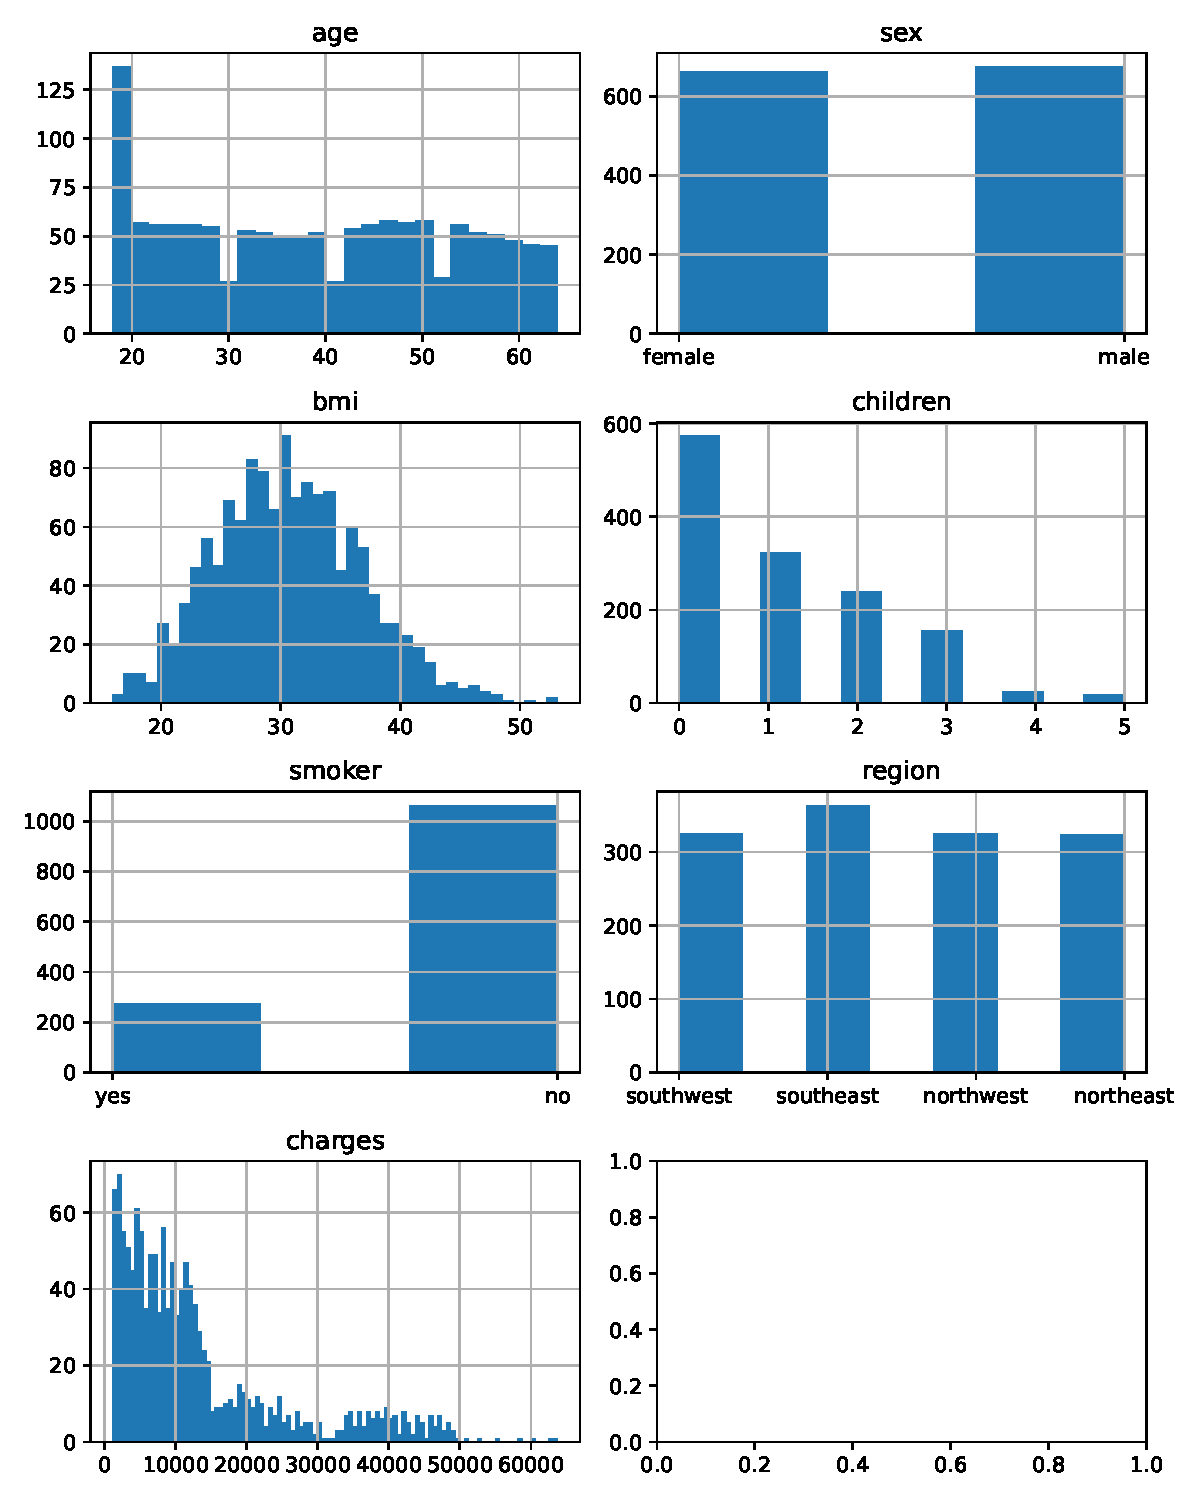
\includegraphics[width=0.95\textwidth]{../figures/variable_distributions.pdf}
  \caption{Distribution of the main predictor variables and the target variable.}
\end{figure}

\section{Relationship Between Predictors and Charges}
The relationship between insurance charges and individual variables was explored through scatter plots and summary comparisons. The strongest visible pattern was observed for smoking status, where smokers exhibited markedly higher charges. Age and BMI showed positive trends, though the relationships were not as dominant as the smoking effect. The variables for sex and region did not reveal strong standalone patterns, suggesting that their influence is likely secondary or interactive rather than direct.

\begin{figure}[H]
  \centering
  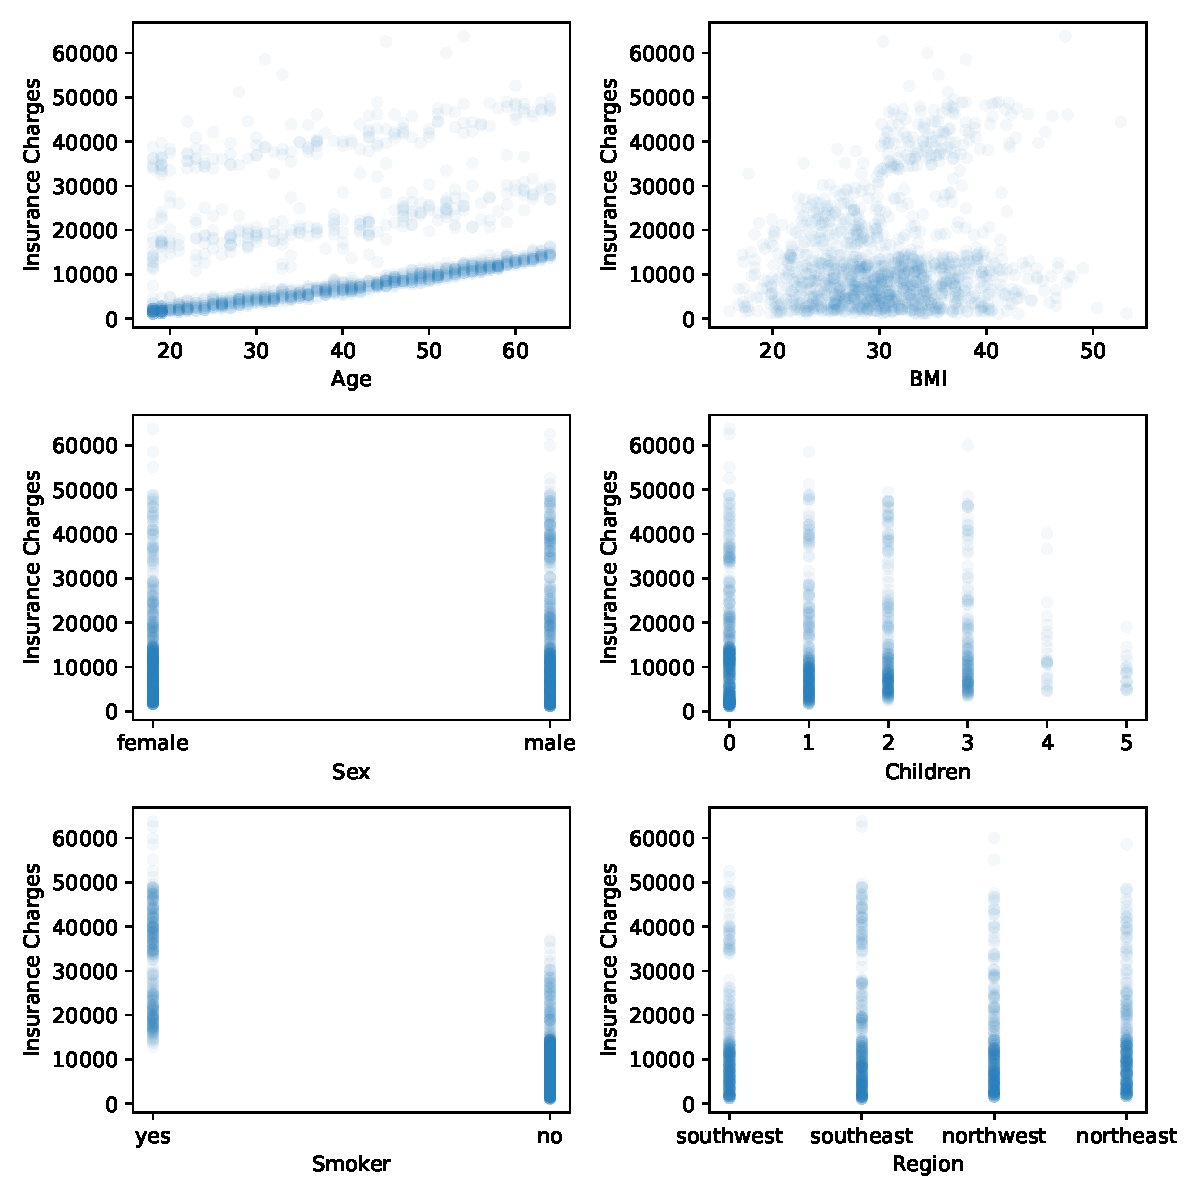
\includegraphics[width=0.95\textwidth]{../figures/insurance_cost_vs_variables.pdf}
  \caption{Insurance charges plotted against key variables to examine their individual relationships.}
\end{figure}

The correlation analysis further supported this interpretation. Although age and BMI showed moderate positive associations with charges, the overall evidence suggested that no single variable alone explains the target sufficiently. This motivates the use of flexible models that can capture non-linear patterns and interactions among predictors.

\begin{figure}[H]
  \centering
  
\includegraphics[width=0.95\textwidth]{../figures/variable_correlations.pdf}
  \caption{Correlation structure among the numerical variables and the target variable.}
\end{figure}

\chapter{Model Development and Evaluation}
\section{Regression Models Compared}
Several regression models were trained and compared to determine the most suitable approach for this problem. The models considered in this study include:
\begin{itemize}
  \item Random Forest Regressor;
  \item Gradient Boosting variants;
  \item Elastic Net regression; and
  \item a Stacking Regressor that combines multiple base estimators.
\end{itemize}

The evaluation process focused on three metrics: mean absolute error (MAE), root mean squared error (RMSE), and the coefficient of determination ($R^2$). These metrics provide complementary information: MAE measures average prediction error, RMSE penalises larger errors more heavily, and $R^2$ indicates how much of the variance in insurance charges is explained by the model.

\begin{table}[H]
  \centering
  \caption{Performance comparison of the evaluated regression models.}
  \begin{tabular}{lccc}
    \toprule
    Model & MAE & RMSE & $R^2$ \\
    \midrule
    Random Forest Regressor & 2534.45 & 4590.44 & 0.8643 \\
    Standard Gradient Boosting & 2447.17 & 4352.16 & 0.8780 \\
    Hist Gradient Boosting & 2609.08 & 4599.76 & 0.8637 \\
    Tuned Gradient Boosting & 2447.17 & 4352.16 & 0.8780 \\
    Elastic Net & -- & 5800.78 & 0.7833 \\
    Stacking Regressor & 2416.36 & 4319.32 & 0.8798 \\
    \bottomrule
  \end{tabular}
\end{table}

\section{Model Interpretation}
The results indicate that the boosted tree models performed better than the linear Elastic Net baseline. This is consistent with the presence of non-linear relationships and interactions between features such as age, BMI, and smoking behaviour. The stacked model achieved the best overall performance by combining the strengths of several base learners, resulting in the lowest MAE and RMSE and the highest $R^2$.

\begin{figure}[H]
  \centering
  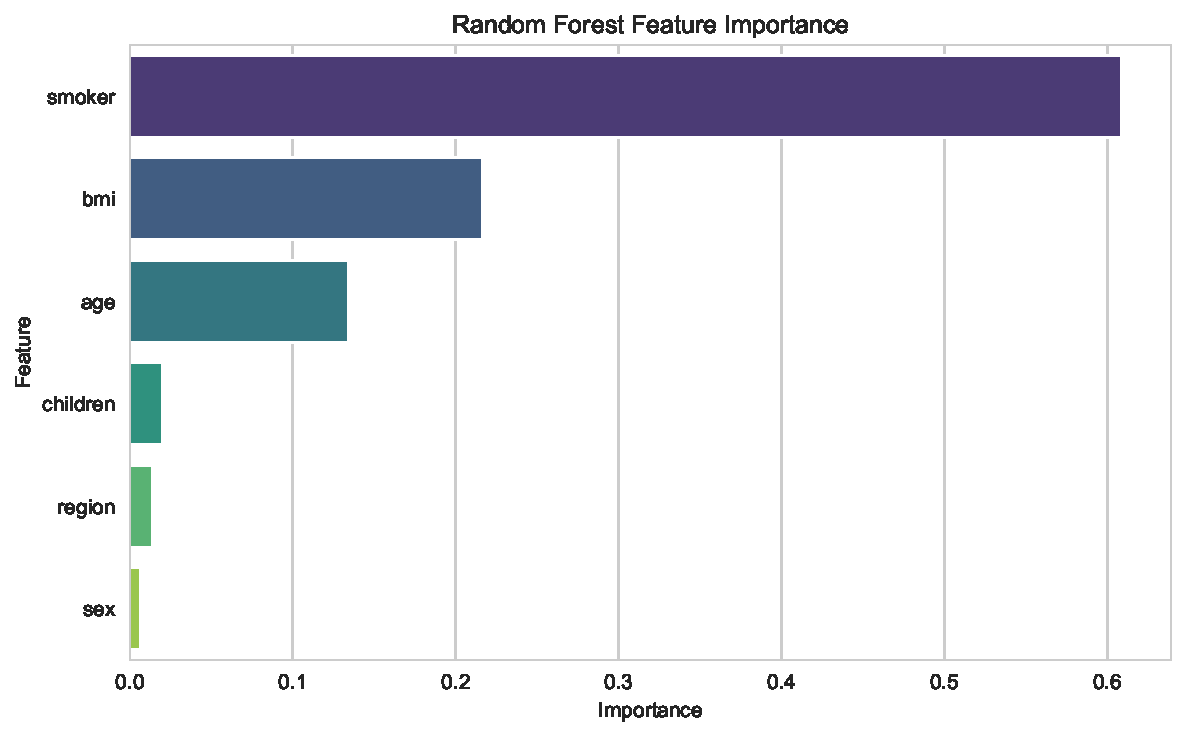
\includegraphics[width=0.95\textwidth]{../figures/random_forest_feature_importance.pdf}
  \caption{Feature importance profile from the tree-based regression analysis.}
\end{figure}

\begin{figure}[H]
  \centering
  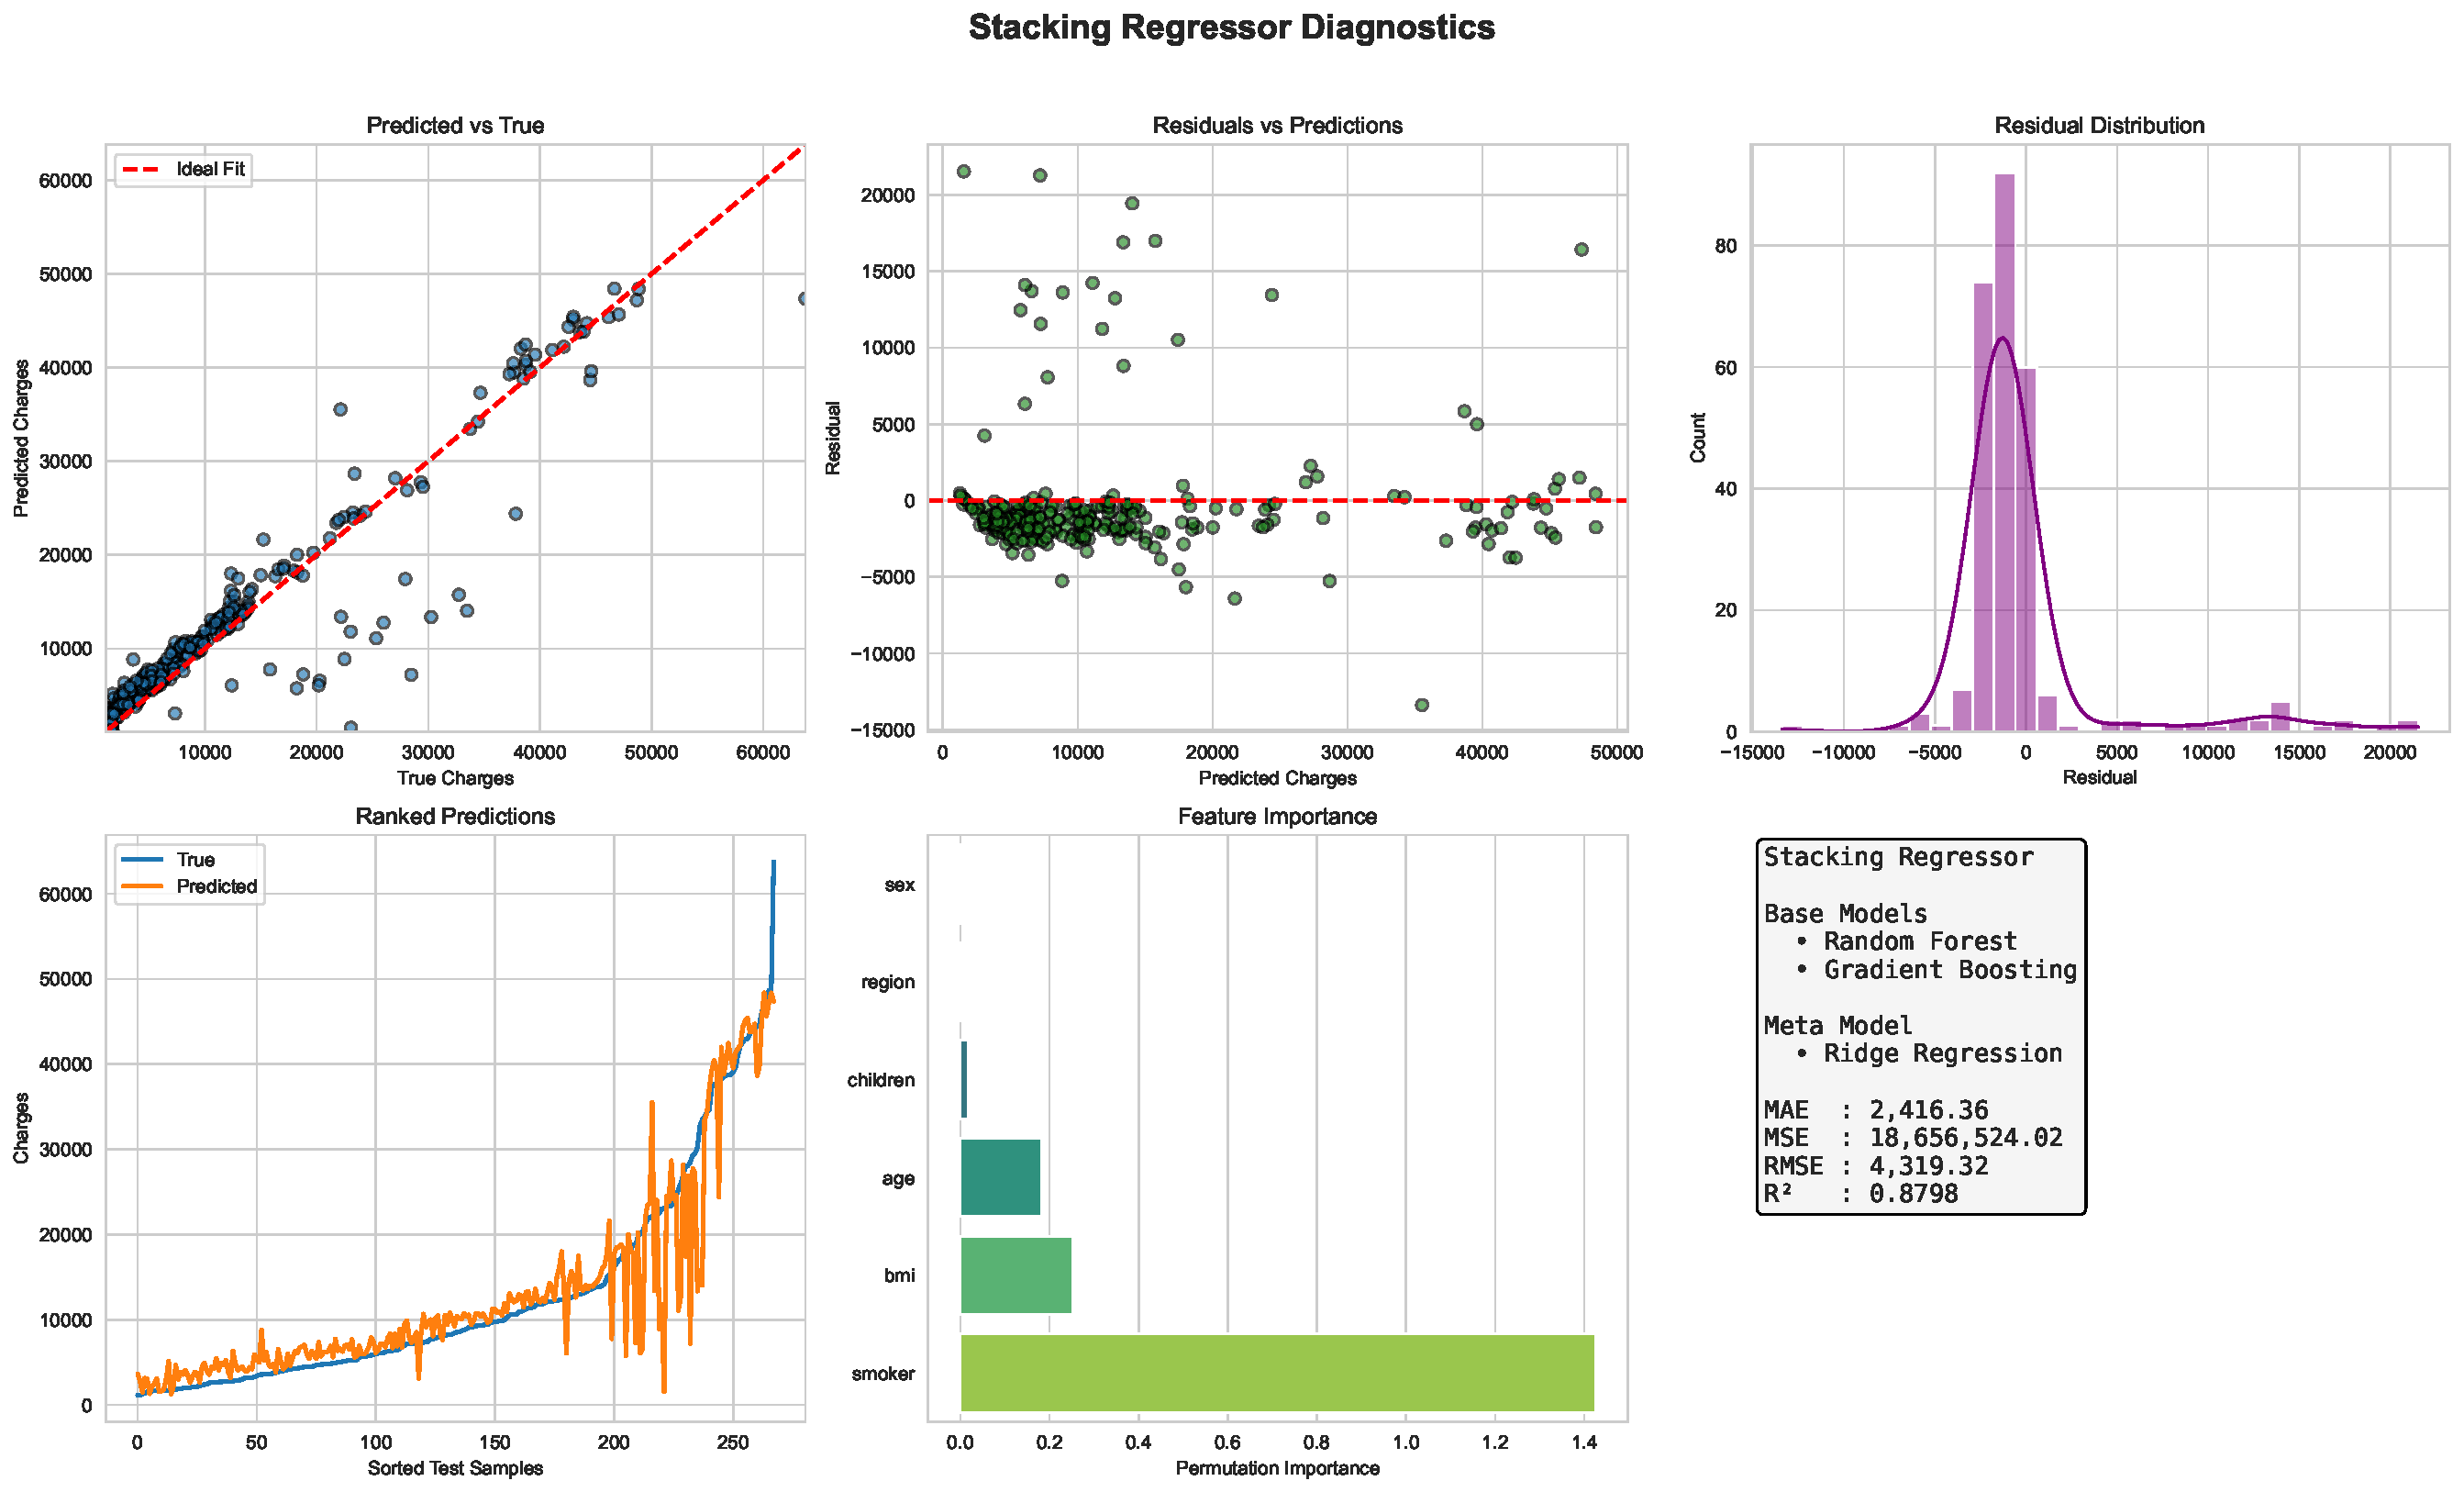
\includegraphics[width=0.95\textwidth]{../figures/stacking_regressor_diagnostics.pdf}
  \caption{Diagnostic plots for the stacked regression model, including residual behaviour and prediction quality.}
\end{figure}

\chapter{Discussion}
The strongest insight from this analysis is that smoking status is the dominant predictor of insurance cost. Individuals who smoke are associated with substantially higher medical expenses, which is consistent with the well-known impact of smoking on health outcomes and healthcare utilisation. Age and BMI also contribute positively, though their influence is less pronounced than smoking behaviour.

The comparison of models demonstrates that tree-based ensemble methods are better suited to this dataset than a purely linear model. The performance gap between Elastic Net and the ensemble methods suggests that the relationships between features and charges are not well captured by a simple linear assumption. The stacking regressor performed best because it aggregates multiple decision-making patterns and reduces the risk of over-reliance on one modelling strategy.

Despite the strong performance of the best model, the residual analysis indicates that the highest-cost cases remain challenging to predict accurately. This may be due to the skewed distribution of charges and the presence of rare but extreme observations. Future work could explore transformations of the target variable, more advanced ensemble strategies, or additional domain features to improve performance further.

\chapter{Conclusion}
This project successfully developed and evaluated a machine learning regression workflow for medical insurance cost prediction. The study demonstrated that insurance charges can be estimated with reasonable accuracy using demographic and health-related features, and that smoking status is the most influential predictor. Among the models tested, the stacking regressor provided the best overall results, achieving an $R^2$ of approximately 0.88 and the lowest error metrics.

Overall, the investigation confirms that regression-based methods can provide valuable predictive insight for insurance pricing and that careful model comparison is essential when the target variable reflects complex and non-linear relationships.
